\addcontentsline{toc}{section}{Introduction}
\section*{Introduction}

Dans ce chapitre, nous explorerons la schématisation détaillée du projet visant à remplacer notre architecture monolithique par une approche basée sur des microservices et des micro-frontends, tout en migrer notre système de gestion de base de données de MariaDB vers Delta Lake. Cette transition marque une étape cruciale dans notre parcours d'évolution technologique, offrant des avantages significatifs en termes de flexibilité, d'évolutivité et de maintenabilité.

\section{Solution}

\begin{figure}[H]
\centering
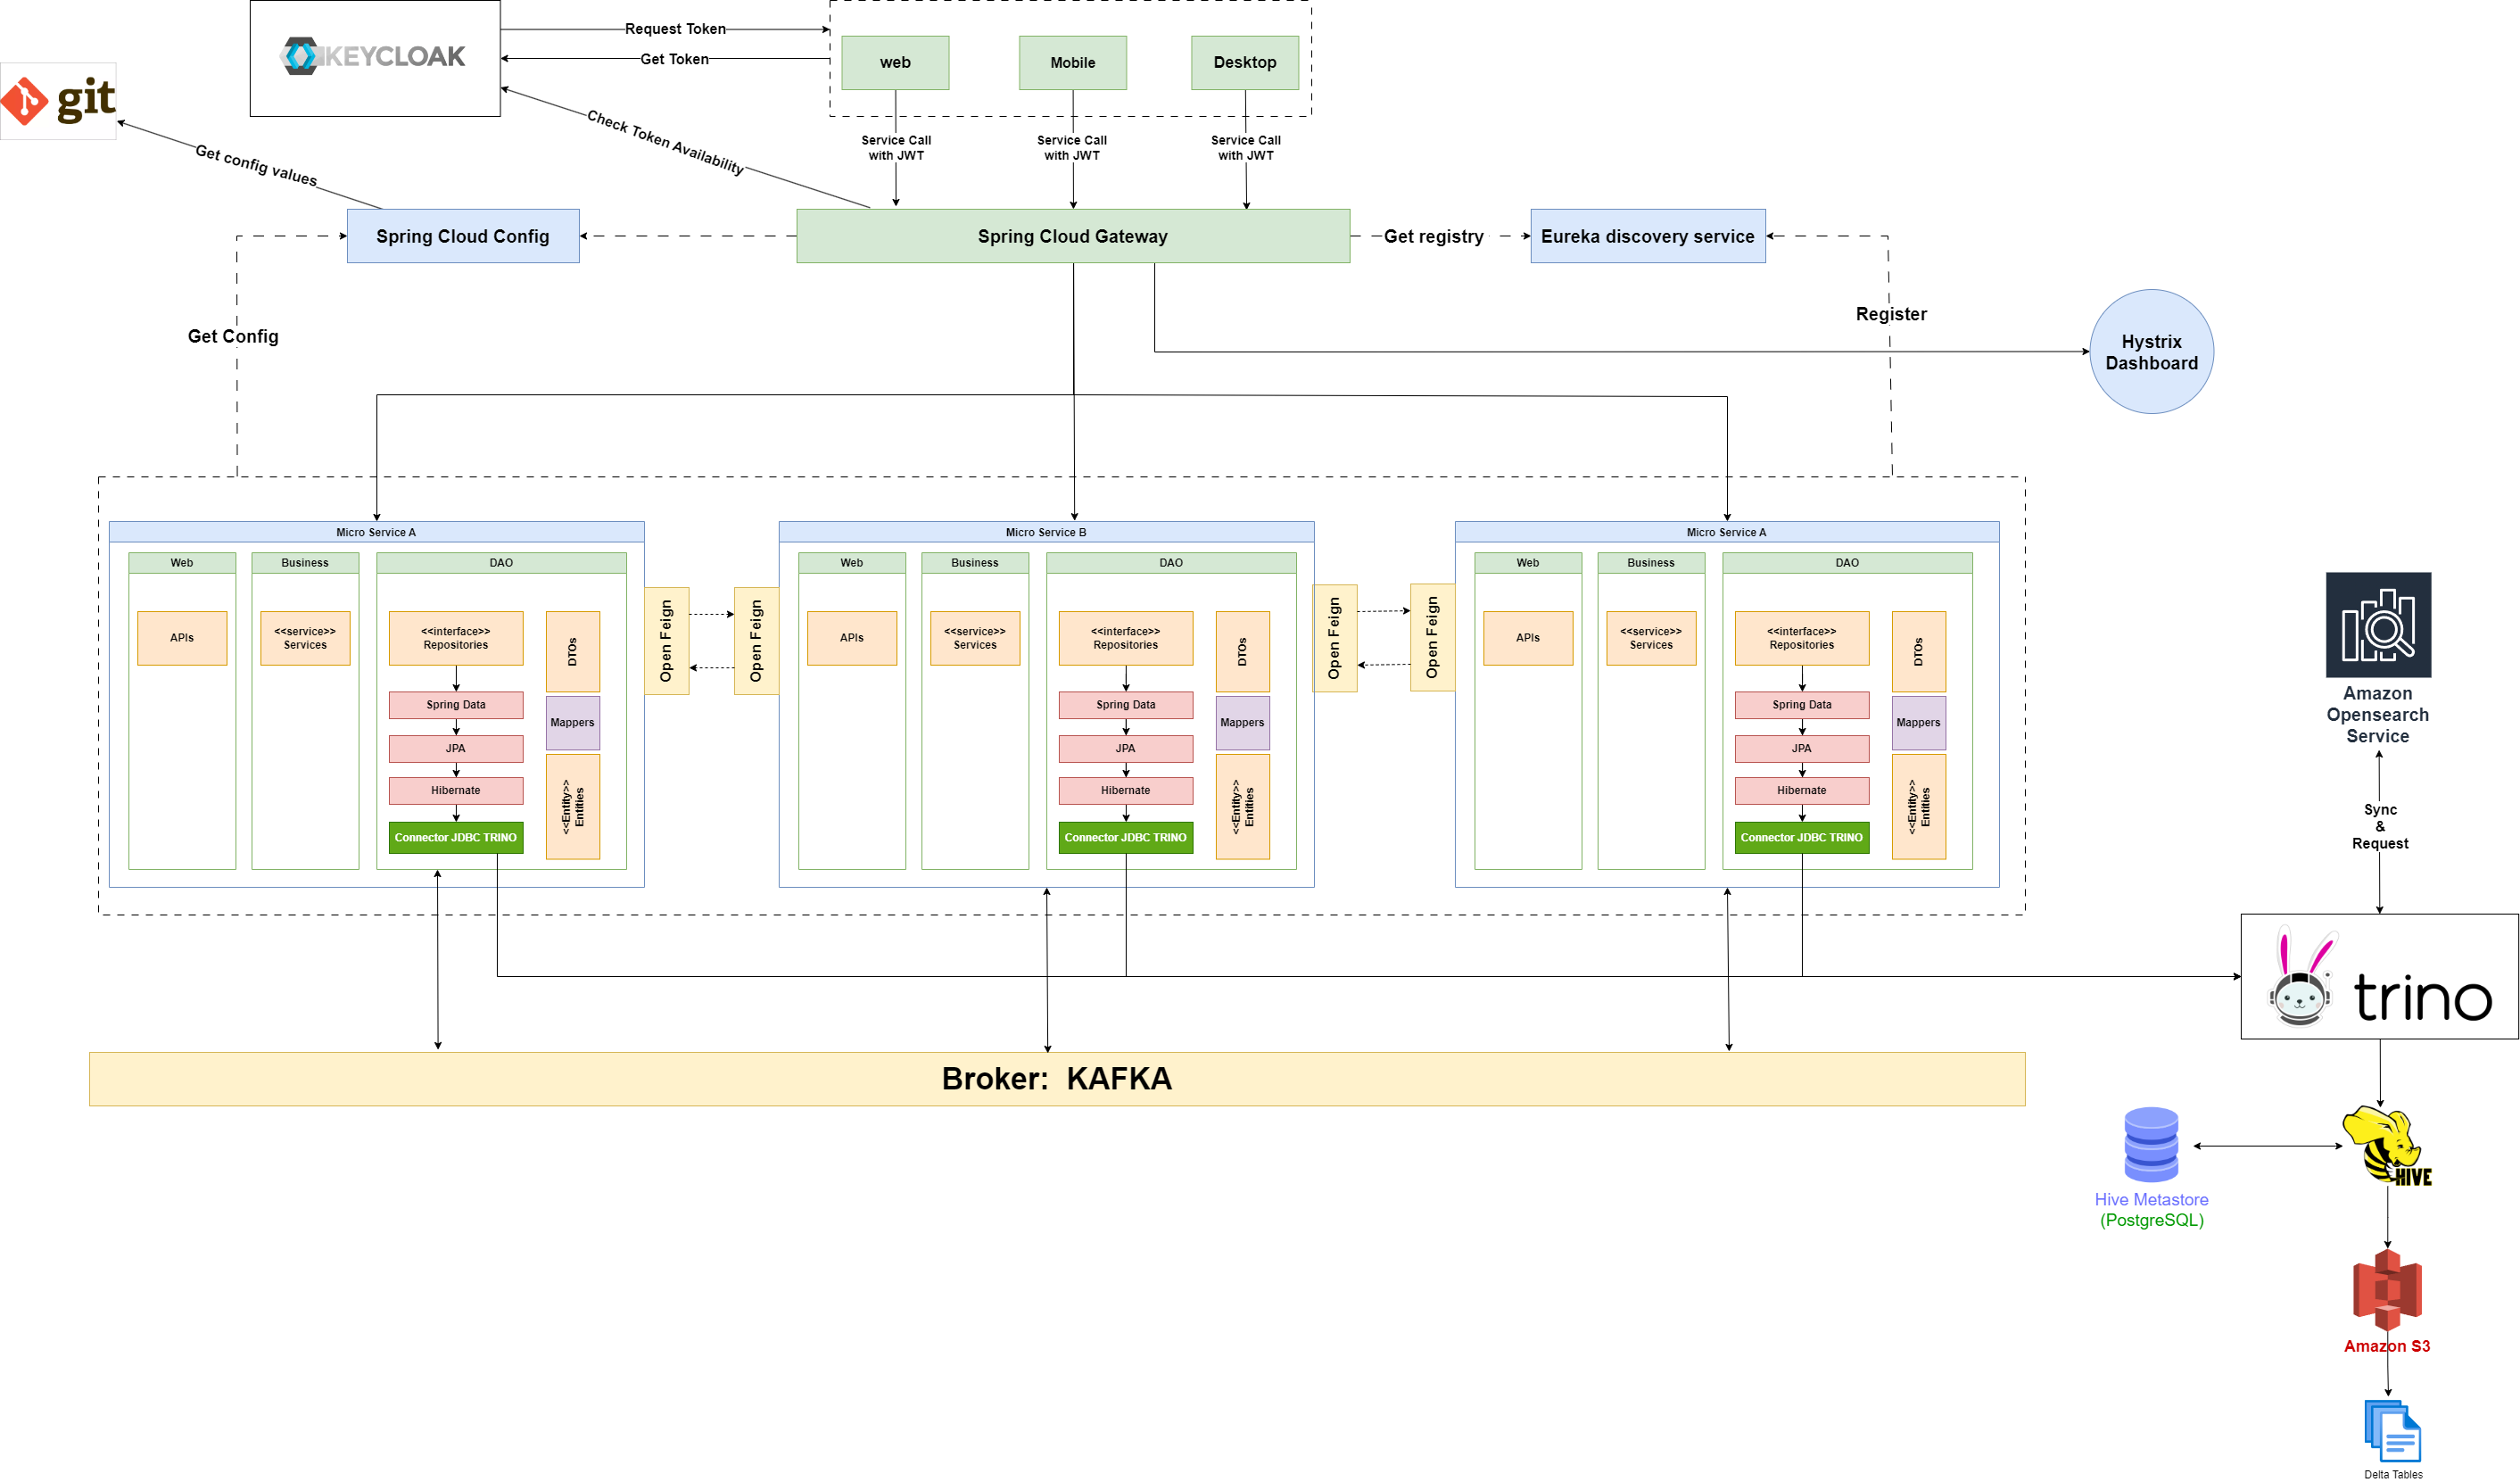
\includegraphics[width=\linewidth]{images/architecture-solution.png}
\caption{Architecture de solution}\label{fig:solution}
\end{figure}

\section*{Conclusion}
\addcontentsline{toc}{section}{Conclusion}

Delta Lake est un outil important pour le traitement du Big Data, fournissant une gestion fiable des données et garantissant l'intégrité des données à grande échelle. Ses transactions ACID, l'application des schémas et les fonctionnalités de gestion des versions des données en font un choix populaire pour les entreprises qui doivent traiter de grandes quantités de données avec une grande précision et fiabilité.

En utilisant Delta Lake, les ingénieurs de données et les scientifiques des données peuvent facilement gérer la qualité des données, suivre la lignée des données et collaborer sur des projets d'analyse de données. Grâce à son intégration transparente avec d'autres outils de Big Data. Delta Lake fournit une solution puissante pour le traitement du Big Data qui peut aider les entreprises à mieux comprendre leurs données plus rapidement et plus efficacement.